\section{Software Infrastructure}

\subsection{Virtualization}

\subsubsection{What is a Virtual Machine?}

A \definition{Virtual Machine (VM)} is a \textbf{logical abstraction} able to \textbf{provide a virtualized execution environment}. More specifically, a VM:
\begin{itemize}
    \item Provides identical software behavior
    \item Consists in a combination of physical machine and virtualizing software
    \item May appear as different resources than physical machine
    \item May result in different level of performances
\end{itemize}
Exists two type of Virtual Machine: Process VM (page \pageref{Process VM}) and System VM (page \pageref{System VM}).

\highspace
\begin{flushleft}
    \textcolor{Green3}{\faIcon{question-circle} \textbf{What's the difference between a physical machine and a virtual machine?}}
\end{flushleft}
First of all, the \textbf{physical machine} is the computer that can \textbf{\emph{host}} $n$ \textbf{virtual machines}. 

\highspace
Furthermore, every VM is based on hypervisor software (also known as a virtual machine manager or monitor VMM, page \pageref{subsubsection: Virtual Machine Managers (VMM)}). The hypervisor runs as an application on the host operating system (hosted hypervisor) or rests directly on the hardware of the physical machine (bare-metal hypervisor) and manages the hardware resources provided by the host system. The \textbf{hypervisor software creates an abstraction layer between physical hardware and virtual machines}. \textbf{Each VM runs isolated from the host system and other guest systems on its own virtual environment}. This is referred to as encapsulation. 

\highspace
Processes within a virtual machine do not affect the host or other VMs on the same hardware.

\highspace
So, to sum up:
\begin{enumerate}
    \item \textbf{Physical machines} are the computers that can \textbf{\emph{host}} $n$ \textbf{virtual machines}.
    
    \item Each \textbf{physical machine has a hypervisor (VMM)} already enabled or asleep on the hardware. \textbf{It manages the resources made available by the physical machine}.
    
    \item Each \textbf{virtual machine has its own virtual environment}, so they are \textbf{encapsulated}, \textbf{isolated environments.} 
    
    Obviously, the statement is not true if there is a \dquotes{\emph{virtual machine escape attack}}, but we don't count those extreme cases.\cite{wu2017access}
\end{enumerate}

\newpage

\begin{figure}[!htp]
    \centering
    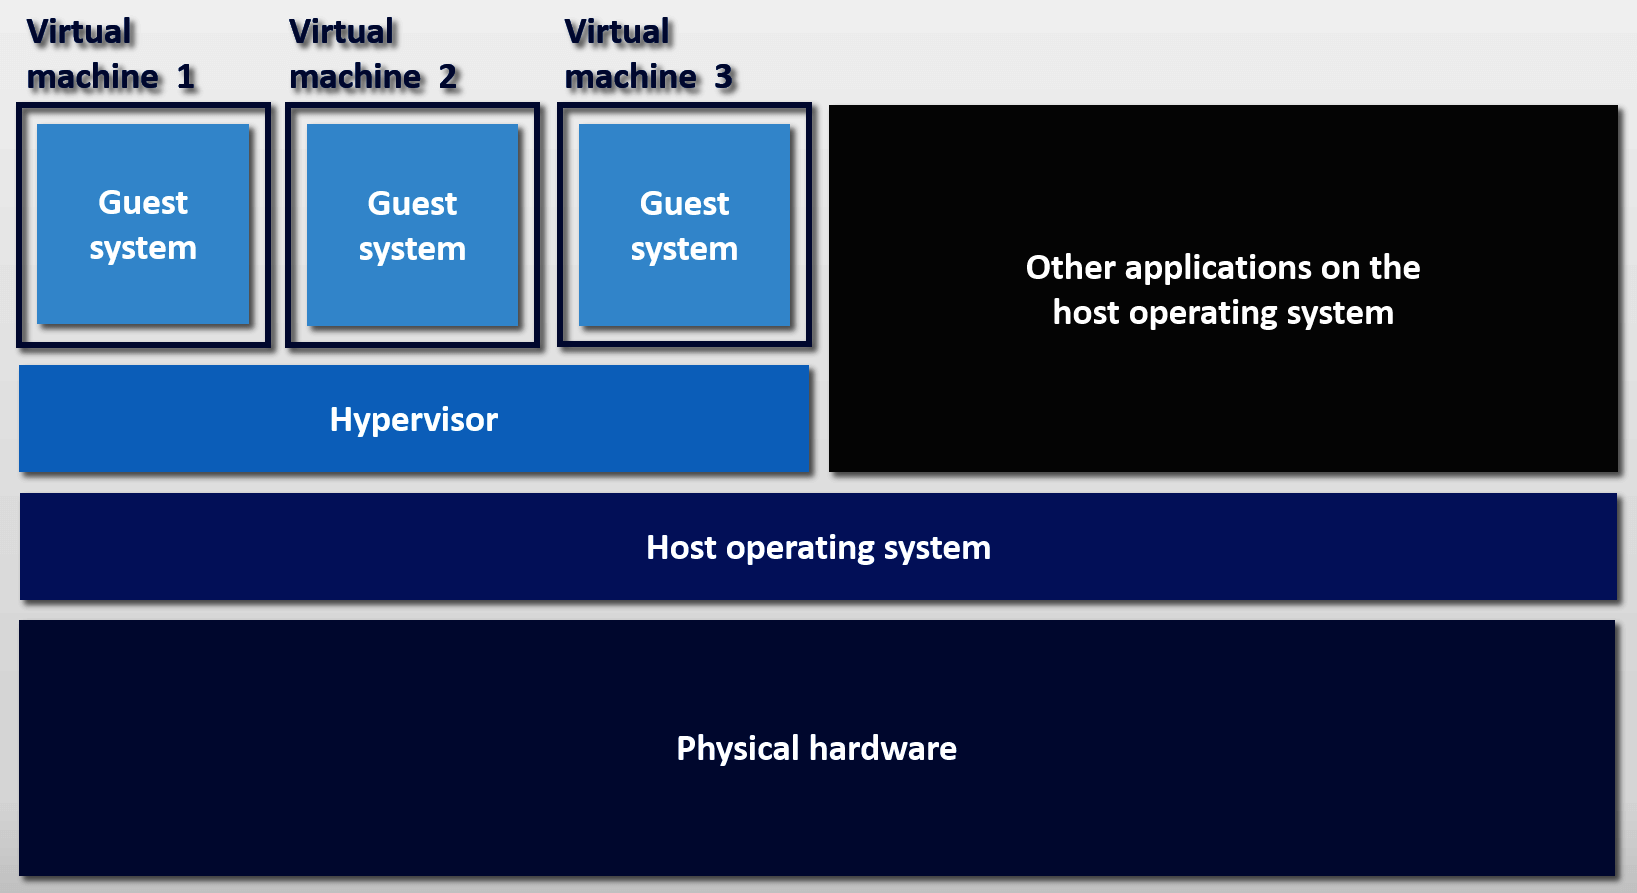
\includegraphics[width=\textwidth]{img/vm-1.png}
    \caption{Operating system view if there are VMs in the physical machine (source: \href{https://www.ionos.co.uk/digitalguide/server/know-how/virtual-machines/}{ionos}).}
\end{figure}

\noindent
A little terminology about \emph{host} and \emph{guest}:
\begin{itemize}
    \item \textbf{\underline{Host}}: the underlying platform supporting the environment/system.
    \item \textbf{\underline{Guest}}: the software that runs in the Virtual Machine environment as the guest.
\end{itemize}

\newpage

\paragraph{Process VM}\label{Process VM}

A \definition{Process Virtual Machine}, sometimes called an application virtual machine, or Managed Runtime Environment (MRE), \textbf{runs as a normal application inside a host OS and supports a single process}. 

\highspace
The \textbf{Virtual Machine is created when that process begins and destroyed when it ends}. A good example is the Java Virtual Machine JVM (see more \href{https://en.wikipedia.org/wiki/Java_virtual_machine}{here}).

\highspace
The purpose of a process VM is to execute a computer program in a platform-independent environment, meaning it can run on a variety of hardware or software.

\highspace
The virtualizing software:
\begin{itemize}
    \item is placed at the ABI\footnote{An \definition{Application Binary Interface (ABI)} corresponds to \dquotes{\emph{Operating system machine level}}.}, on top of the OS/hardware combination.
    \item emulates both user-level instructions and operating system calls.
    \item is usually called Runtime Software.
\end{itemize}

\begin{figure}[!htp]
    \centering
    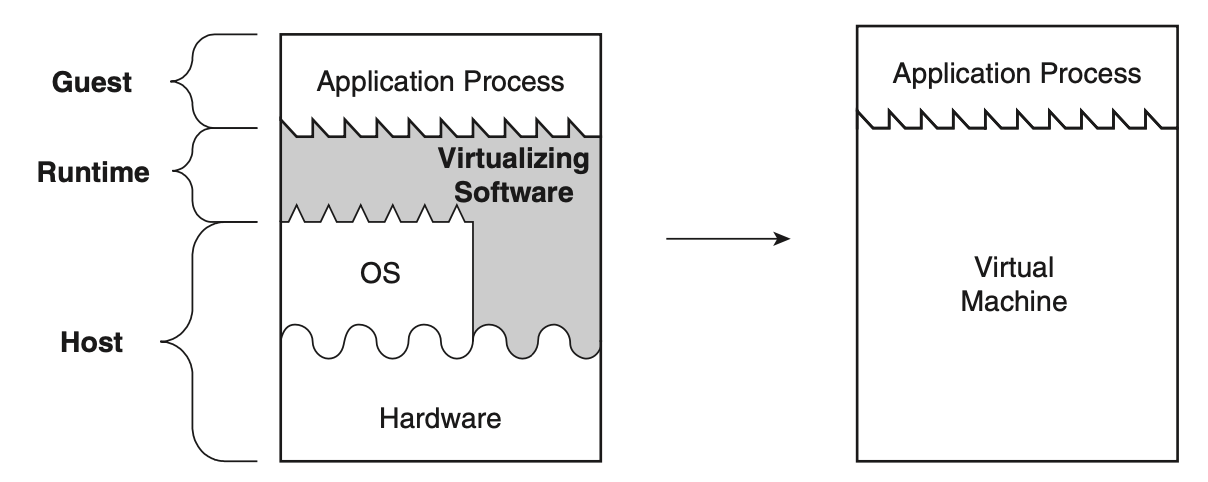
\includegraphics[width=.9\textwidth]{img/vm-2.png}
    \caption{Process VM.}
\end{figure}

\newpage

\paragraph{System VM}\label{System VM}

\definition{System Virtual Machine}s are substitutes for real machines and \textbf{provide all the functionalities of an actual operating system}. It provides operating system running in it access to underlying hardware resources (networking, I/O, GUI).

\highspace
With a system VM, the hypervisor will access the underlying machine's resources, giving the user the same capabilities the host device offers.

\highspace
The \textbf{virtualization software is called \definition{Virtual Machine Monitor (VMM)}}.

\begin{figure}[!htp]
    \centering
    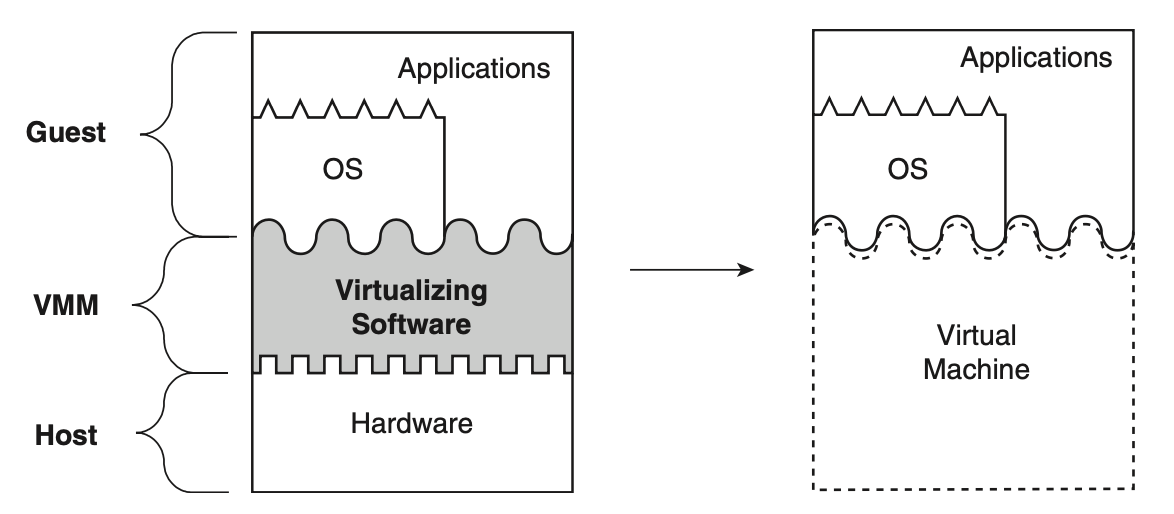
\includegraphics[width=.9\textwidth]{img/vm-3.png}
    \caption{System VM.}
\end{figure}

\newpage

\subsubsection{Virtualization Implementation}

Consider a typical layered architecture of a system by adding layers between layers of the execution stack. Depending on where the new layer is placed, we get different types of virtualization. The virtualization technologies are:
\begin{itemize}
    \item \definition{Hardware-level virtualization}. The \textbf{virtualization layer is placed between hardware and OS}. The interface seen by OS and application might be different from the physical one.
    
    \item \definition{Application-level virtualization}. The \textbf{virtualization layer is placed between the OS and some application} (e.g. JVM). It provides the same interface to the applications. The applications run in their environment, \emph{independently} from OS.
    
    \item \definition{System-level virtualization}. The \textbf{virtualization layers provides the interface of a physical machine to a secondary OS and a set of application running in it, allowing them to run on top of an existing OS}. It is placed between the system's OS and other OS (e.g. VMware, VirtualBox). We can enable several OSs to run on a single hardware.
\end{itemize}
The properties of virtualization technologies are:
\begin{itemize}
    \item \textbf{\underline{Partitioning}}
    \begin{itemize}
        \item Execution of multiple OSs on a single physical machine;
        \item Partitioning of resources between the different VMs.
    \end{itemize}
    
    \item \textbf{\underline{Isolation}}
    \begin{itemize}
        \item Fault tolerance and security (hardware level);
        \item Advanced resource control to guarantee performance (managed by the hypervisor).
    \end{itemize}
    
    \item \textbf{\underline{Encapsulation}}
    \begin{itemize}
        \item The entire state of a VM can be saved in a file (e.g. freeze and restart the execution);
        \item Because a VM is a file, can be copied/moved as a file.
    \end{itemize}
    
    \item \textbf{\underline{Hardware independence}}
    \begin{itemize}
        \item Provisioning/migration of a given VM on a given physical server.
    \end{itemize}
\end{itemize}

\newpage

\subsubsection{Virtual Machine Managers (VMM)}\label{subsubsection: Virtual Machine Managers (VMM)}

A \definition{Virtual Machine Manager (VMM)} is an application that:
\begin{itemize}
    \item \textbf{Manages} the \textbf{VMs};
    \item \textbf{Mediates access to the hardware resources} on the physical host system;
    \item Intercepts and \textbf{handles} any \textbf{privileged} or \textbf{protected} \textbf{instructions issued by the VMs}.
\end{itemize}
This type of virtualization typically runs virtual machines whose operating system, libraries, and utilities have been compiled for the same type of processor and instruction set as the physical machine on which the virtual systems are running.

\highspace
Note that the Virtual Machine Manager (VMM) can be referred to by different names and also different meanings:
\begin{itemize}
    \item \definition{Virtual Machine Manager (VMM)}. The virtualization software.

    \item \definition{Virtual Machine Monitor}. A virtualization software that runs directly on the hardware.

    \item \definition{Hypervisor}. A VMM or Hypervisor that is also used to create, configure and maintain virtualized resources. It provides a user-friendly interface to the underlying virtualization software.
\end{itemize}

\highspace
There are two types of hypervisor:
\begin{itemize}
	\item \definition{Type 1 Hypervisor} or \definition{Bare Metal Hypervisor} (or \definition{Native Hypervisor}). The term \textbf{\emph{bare metal}} refers to the fact that \textbf{there is no operating system between the virtualization software and the hardware}. The virtualization software resides on the \dquotes{bare metal} or the hard disk of the hardware, where the operating system is usually installed.
	
	Then, the \textbf{hypervisor takes direct control of the hardware}.
	
	\begin{figure}[!htp]
		\centering
		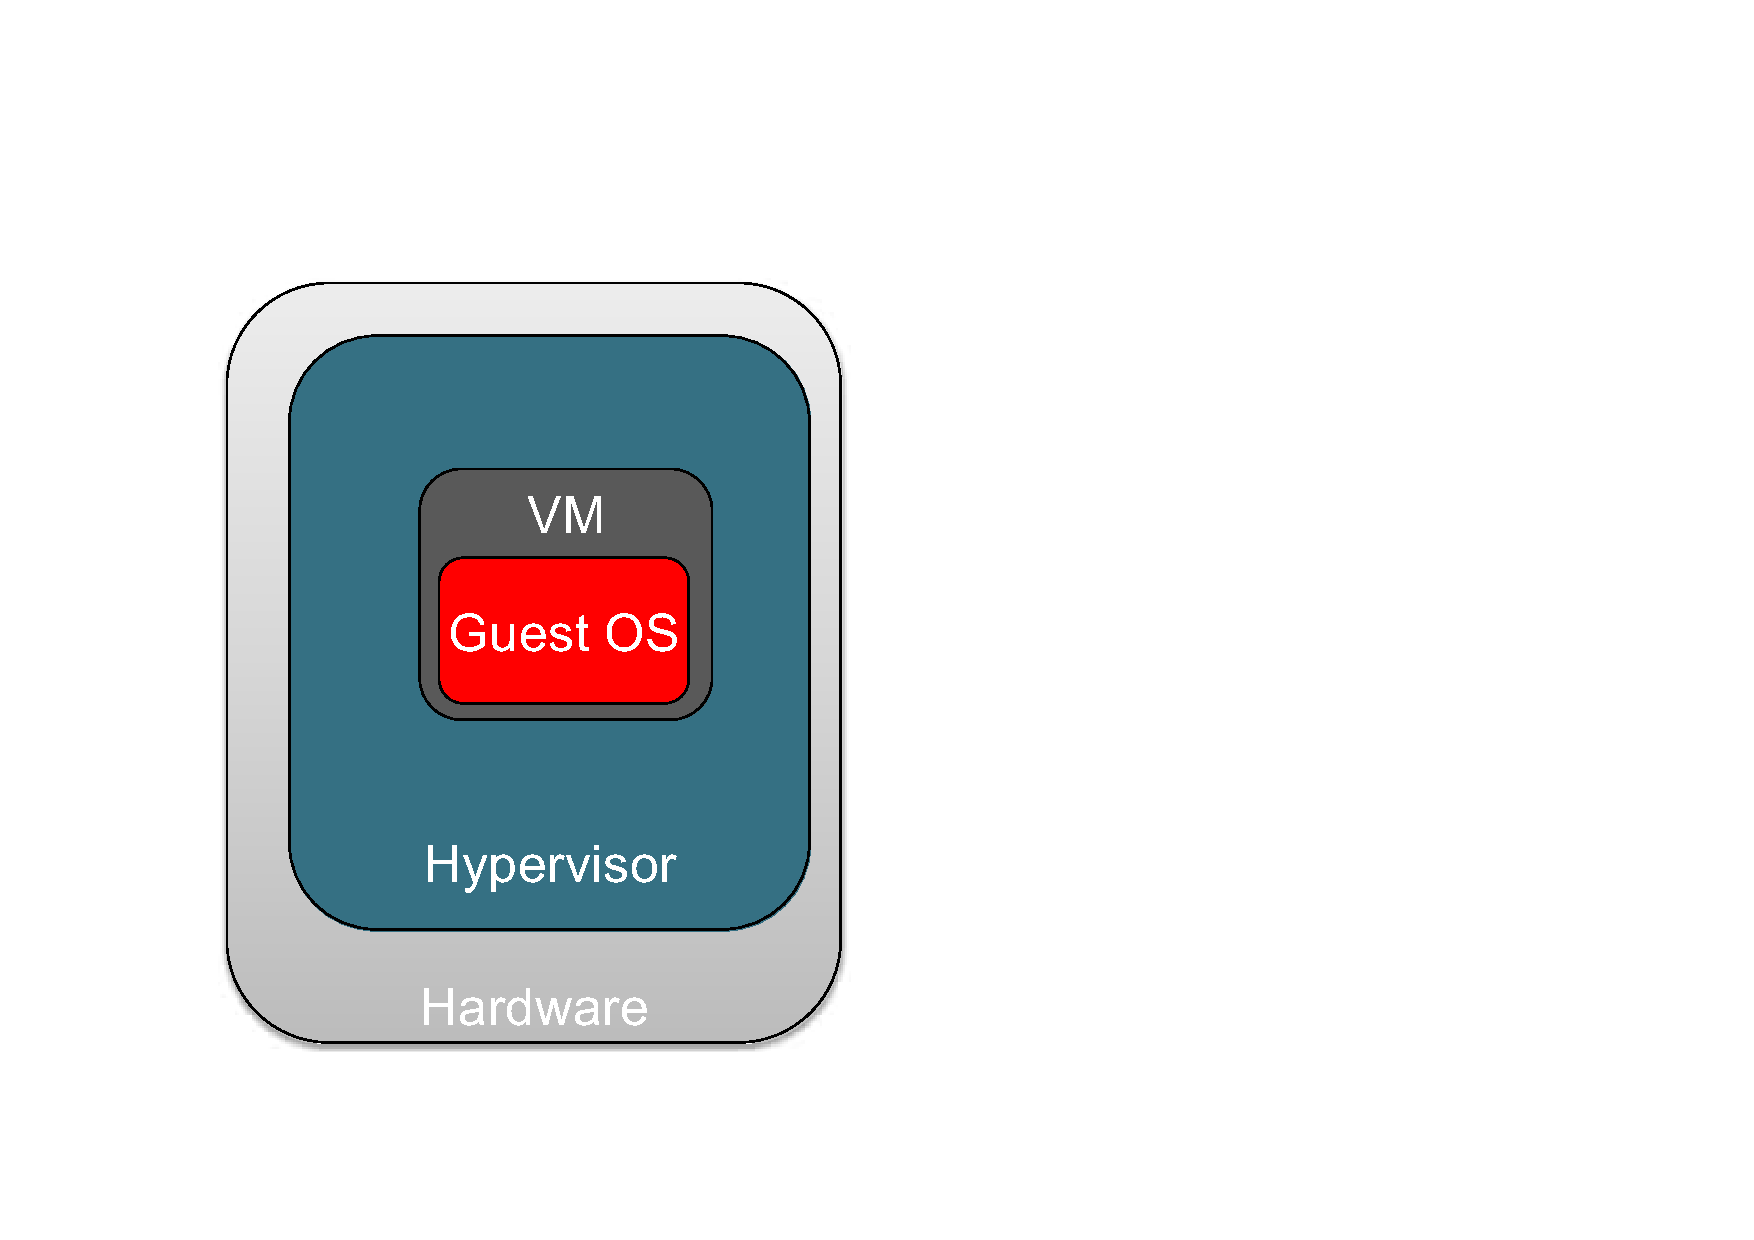
\includegraphics[width=.3\textwidth]{img/vm-4.pdf}
		\caption{View of the Bare Metal Hypervisor.}
	\end{figure}
	\newpage
	Bare Metal Hypervisors can also be \textbf{built in two ways}:
	\begin{itemize}
		\item \definition{Monolithic architecture}. Device \textbf{drivers run within the hypervisor}.
		\begin{flushleft}
			\textcolor{Green3}{\faIcon{check-circle} Advantages}
		\end{flushleft}
		\begin{itemize}
			\item Better \textbf{performance}.
			\item Better \textbf{isolation}.
		\end{itemize}
		\begin{flushleft}
			\textcolor{Red2}{\faIcon{thumbs-down} Disadvantages}
		\end{flushleft}
		\begin{itemize}
			\item Can run only on \textbf{hardware} for which the \textbf{hypervisor has drivers}.
		\end{itemize}
		\begin{figure}[!htp]
			\centering
			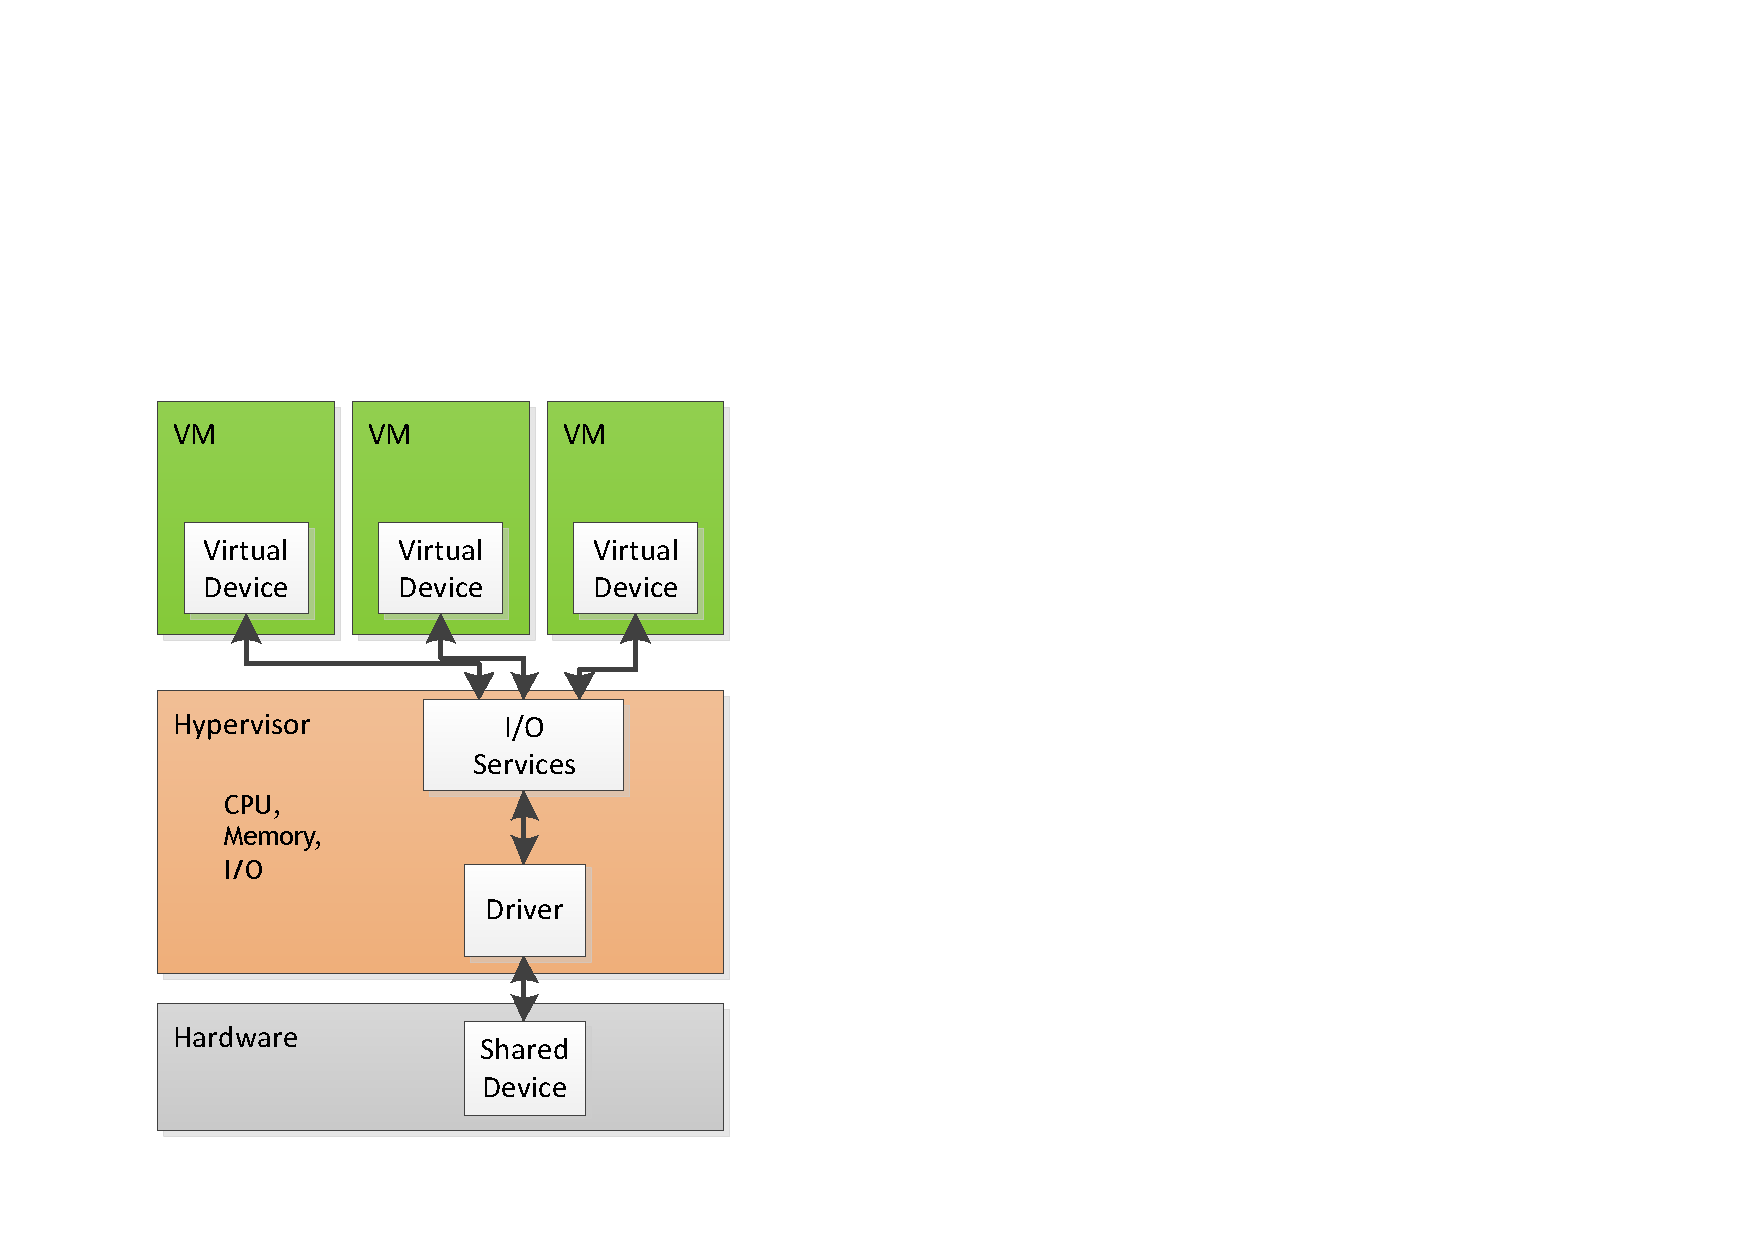
\includegraphics[width=.42\textwidth]{img/vm-5.pdf}
			\caption{Monolithic architecture.}
		\end{figure}
		
		\item \definition{Microkernel architecture}. Device \textbf{drivers run within a service virtual machine}.
		\begin{flushleft}
			\textcolor{Green3}{\faIcon{check-circle} Advantages}
		\end{flushleft}
		\begin{itemize}
			\item \textbf{Smaller hypervisor}.
			\item \textbf{Leverages driver ecosystem} of an existing OS.
			\item Can \textbf{use third party driver} even if not always easy, recompiling might be required.
		\end{itemize}
		\newpage
		\begin{figure}[!htp]
			\centering
			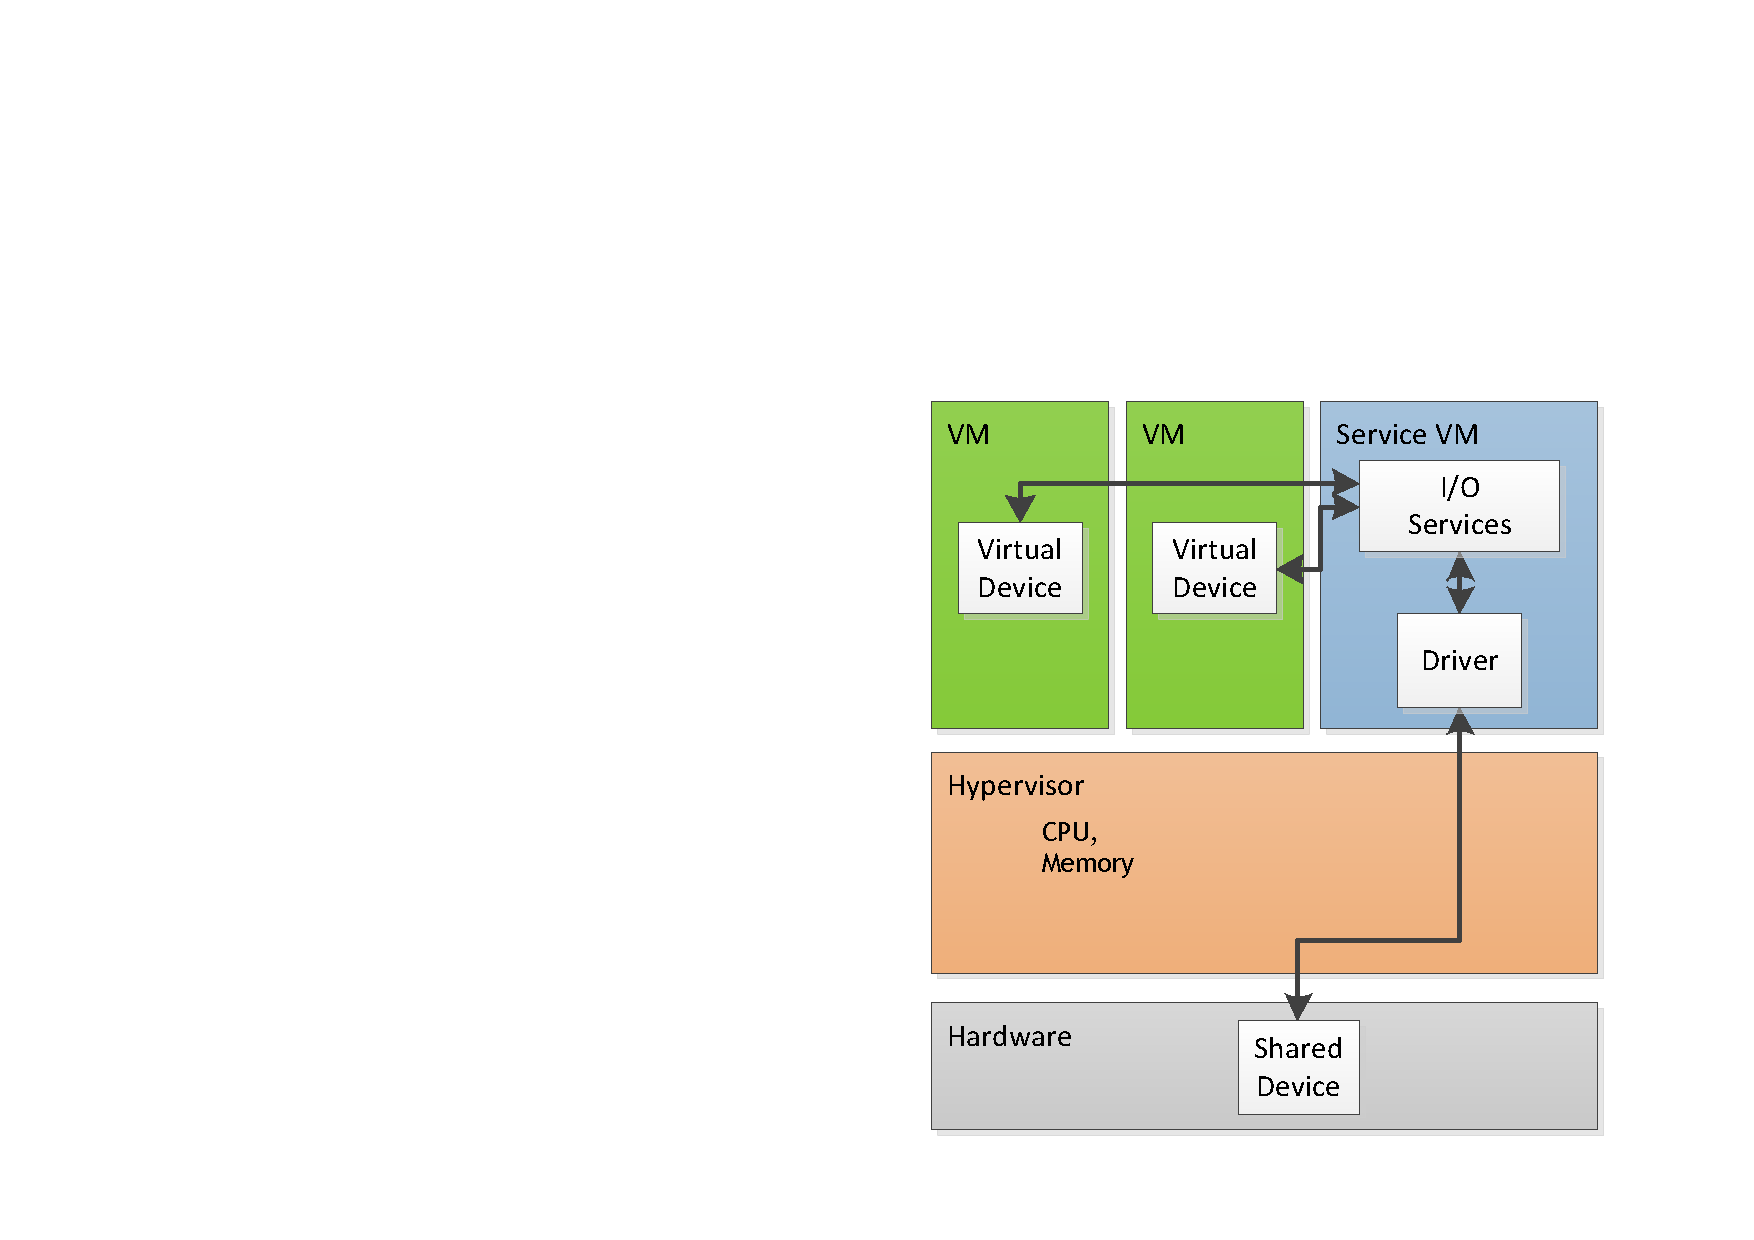
\includegraphics[width=.42\textwidth]{img/vm-6.pdf}
			\caption{Microkernel architecture.}
		\end{figure}
	\end{itemize}


	\item \definition{Type 2 Hypervisor} or \definition{Hosted Hypervisor}. Hosted Hypervisors \textbf{run within the operating system of the host machine}. Although hosted hypervisors run within the OS, additional operating systems can be installed on top of it. Hosted hypervisors have higher latency than bare metal hypervisors because requests between the hardware and the hypervisor must pass through the extra layer of the OS.
	
	This type of hypervisor is also called \emph{hosted hypervisor}. Furthermore, the \emph{Guest OS} is the one that runs in the VM, while applications run in the \emph{Guest 0S}. The \textbf{\emph{Host OS} controls the hardware of the system}.
	\begin{flushleft}
		\textcolor{Green3}{\faIcon{check-circle} Advantages}
	\end{flushleft}
	\begin{itemize}
		\item \textbf{More flexible} in terms of underlying hardware.
		\item \textbf{Simpler} to manage and configure.
	\end{itemize}
	\begin{flushleft}
		\textcolor{Red2}{\faIcon{thumbs-down} Disadvantages}
	\end{flushleft}
	\begin{itemize}
		\item The \emph{Host OS} might \textbf{consume} a non-negligible set of physical \textbf{resources}.
	\end{itemize}
	\begin{figure}[!htp]
		\centering
		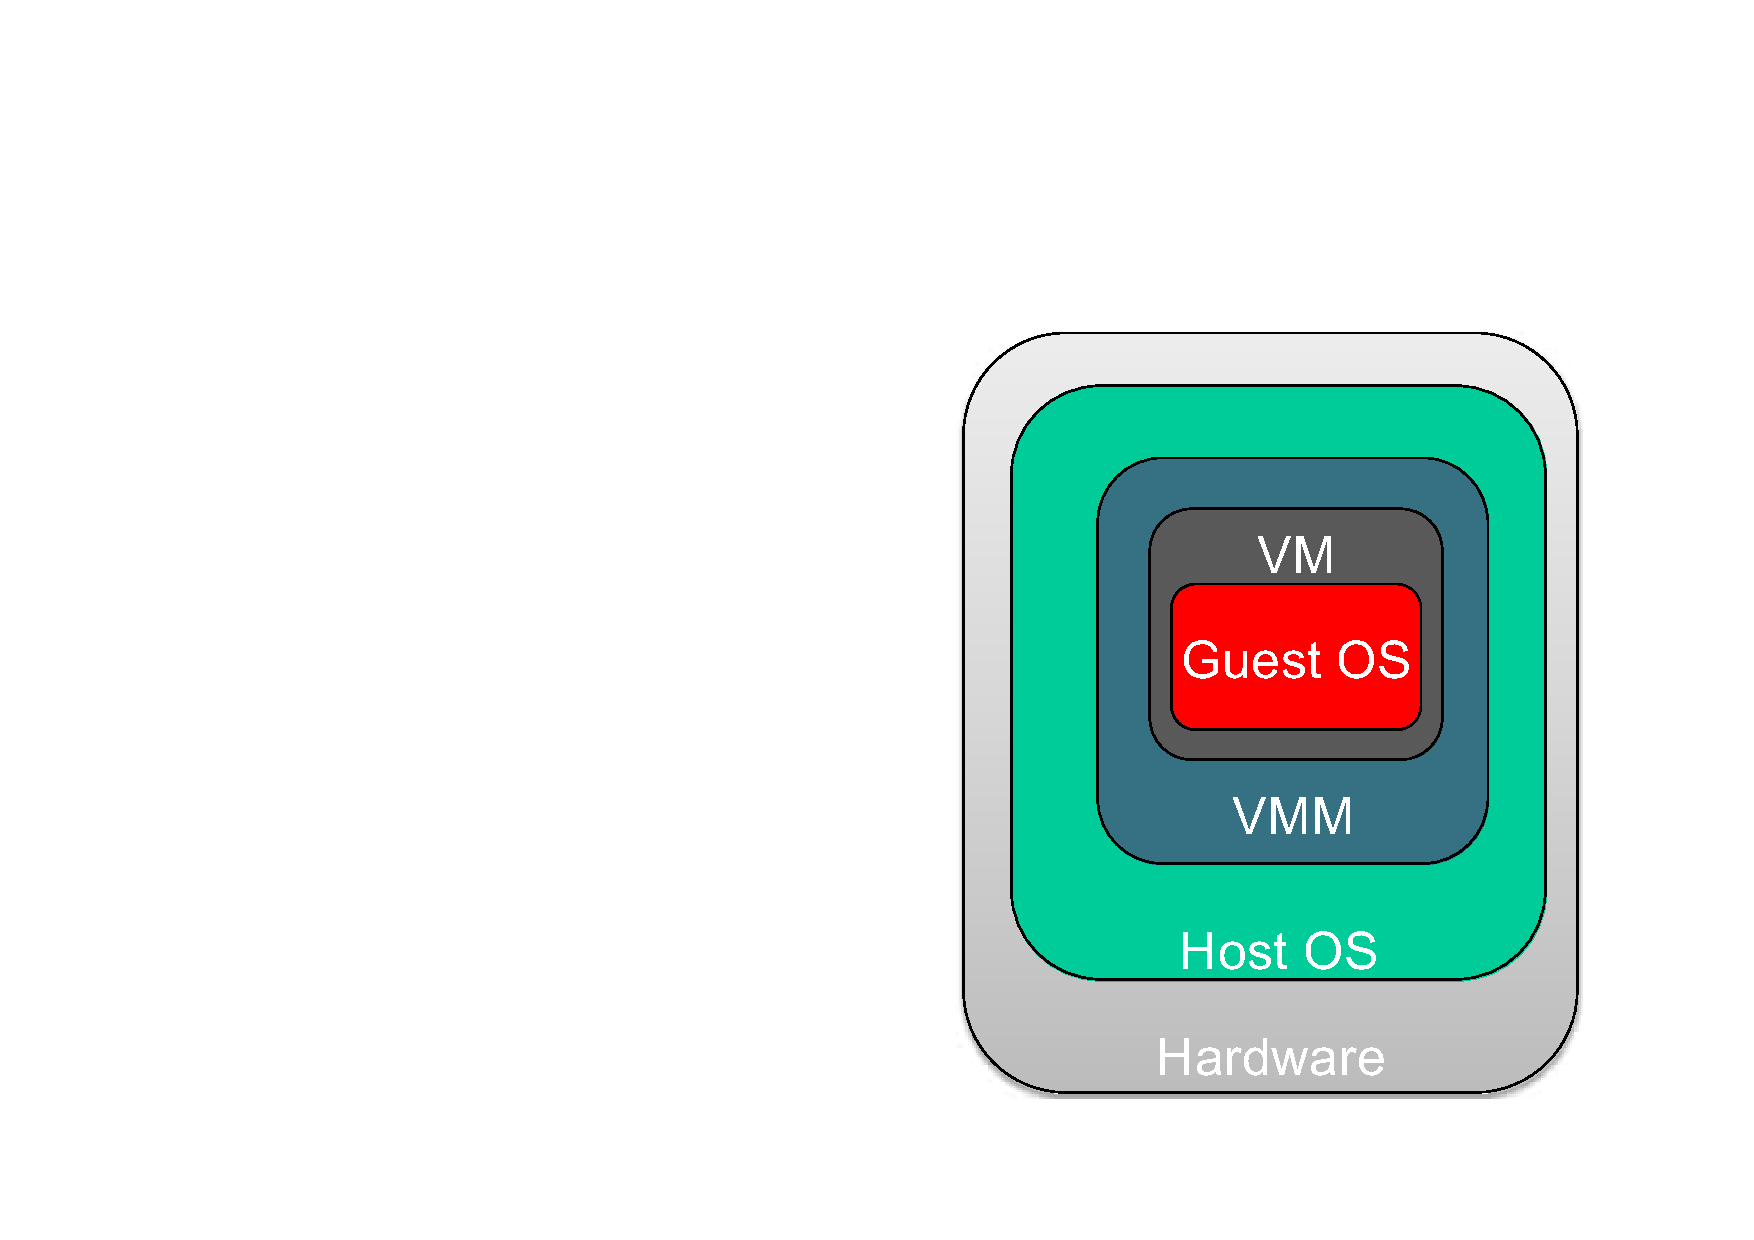
\includegraphics[width=.3\textwidth]{img/vm-7.pdf}
		\caption{View of the Hosted Hypervisor.}
	\end{figure}
\end{itemize}
The data is taken from \href{https://www.vmware.com/topics/bare-metal-hypervisor}{VMware}.

\newpage

\paragraph{Full virtualization}

\definition{Full virtualization} is a virtualization technique that \textbf{provides a complete simulation of the underlying hardware}.

\highspace
In full virtualization, the \textbf{original operating system runs without knowing it's virtualized}, using translation to handle system calls.

\highspace
In full virtualization, the \textbf{virtual machine completely isolates the guest OS from the virtualization layer and hardware}.

\highspace
\begin{flushleft}
	\textcolor{Green3}{\faIcon{check-circle} Advantages}
\end{flushleft}
\begin{itemize}
	\item \textbf{Running unmodified OS}.
	\item \textbf{Complete isolation}.
\end{itemize}

\begin{flushleft}
	\textcolor{Red2}{\faIcon{thumbs-down} Disadvantages}
\end{flushleft}
\begin{itemize}
	\item \textbf{Performance}.
	\item \textbf{Hypervisor mediation} to allow the guest (or guests) and host to request and acknowledge tasks which would otherwise be executed in the virtual domain.
	\item \textbf{Not allowed on all architectures}.
\end{itemize}

\begin{figure}[!htp]
	\centering
	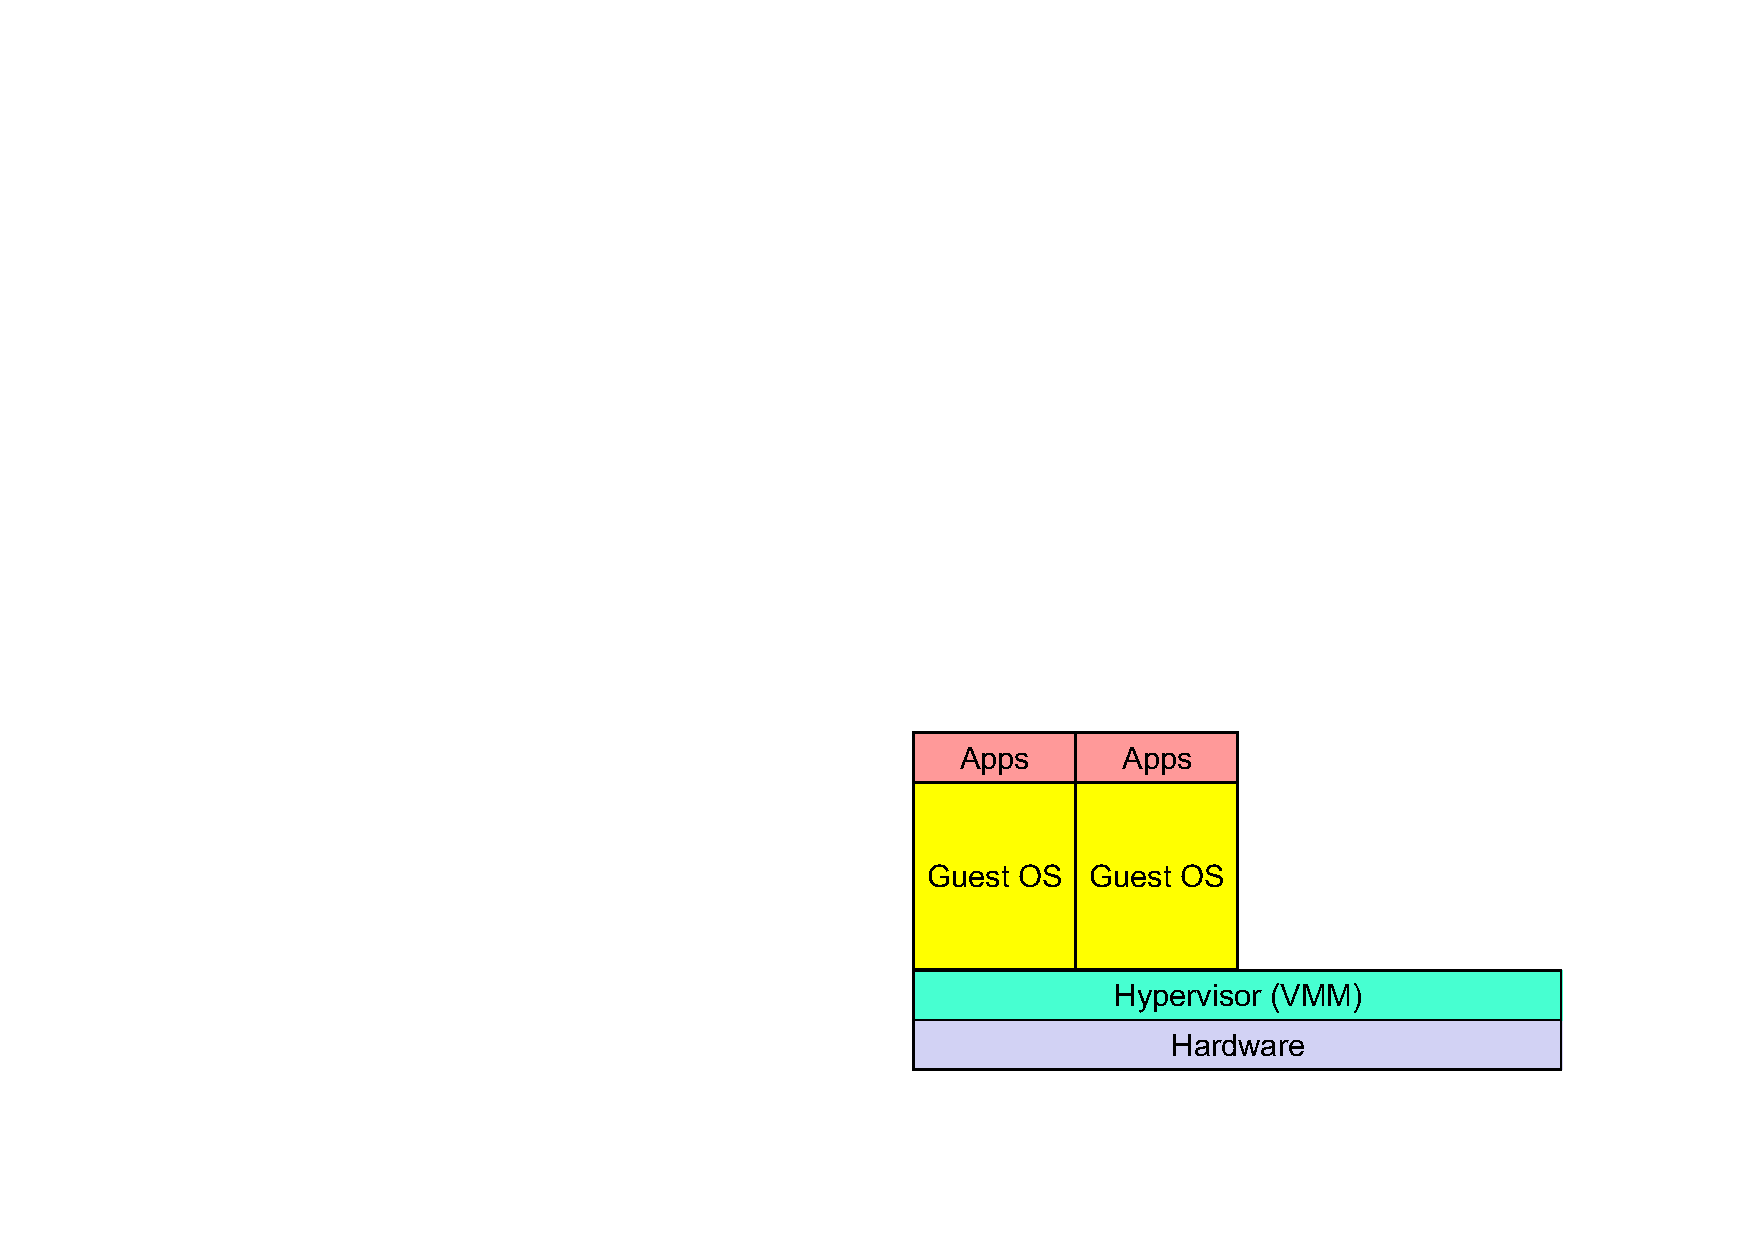
\includegraphics[width=.6\textwidth]{img/full-virtualization-1.pdf}
	\caption{View of the Full Virtualization.}
\end{figure}

\newpage

\begin{figure}[!htp]
	\centering
	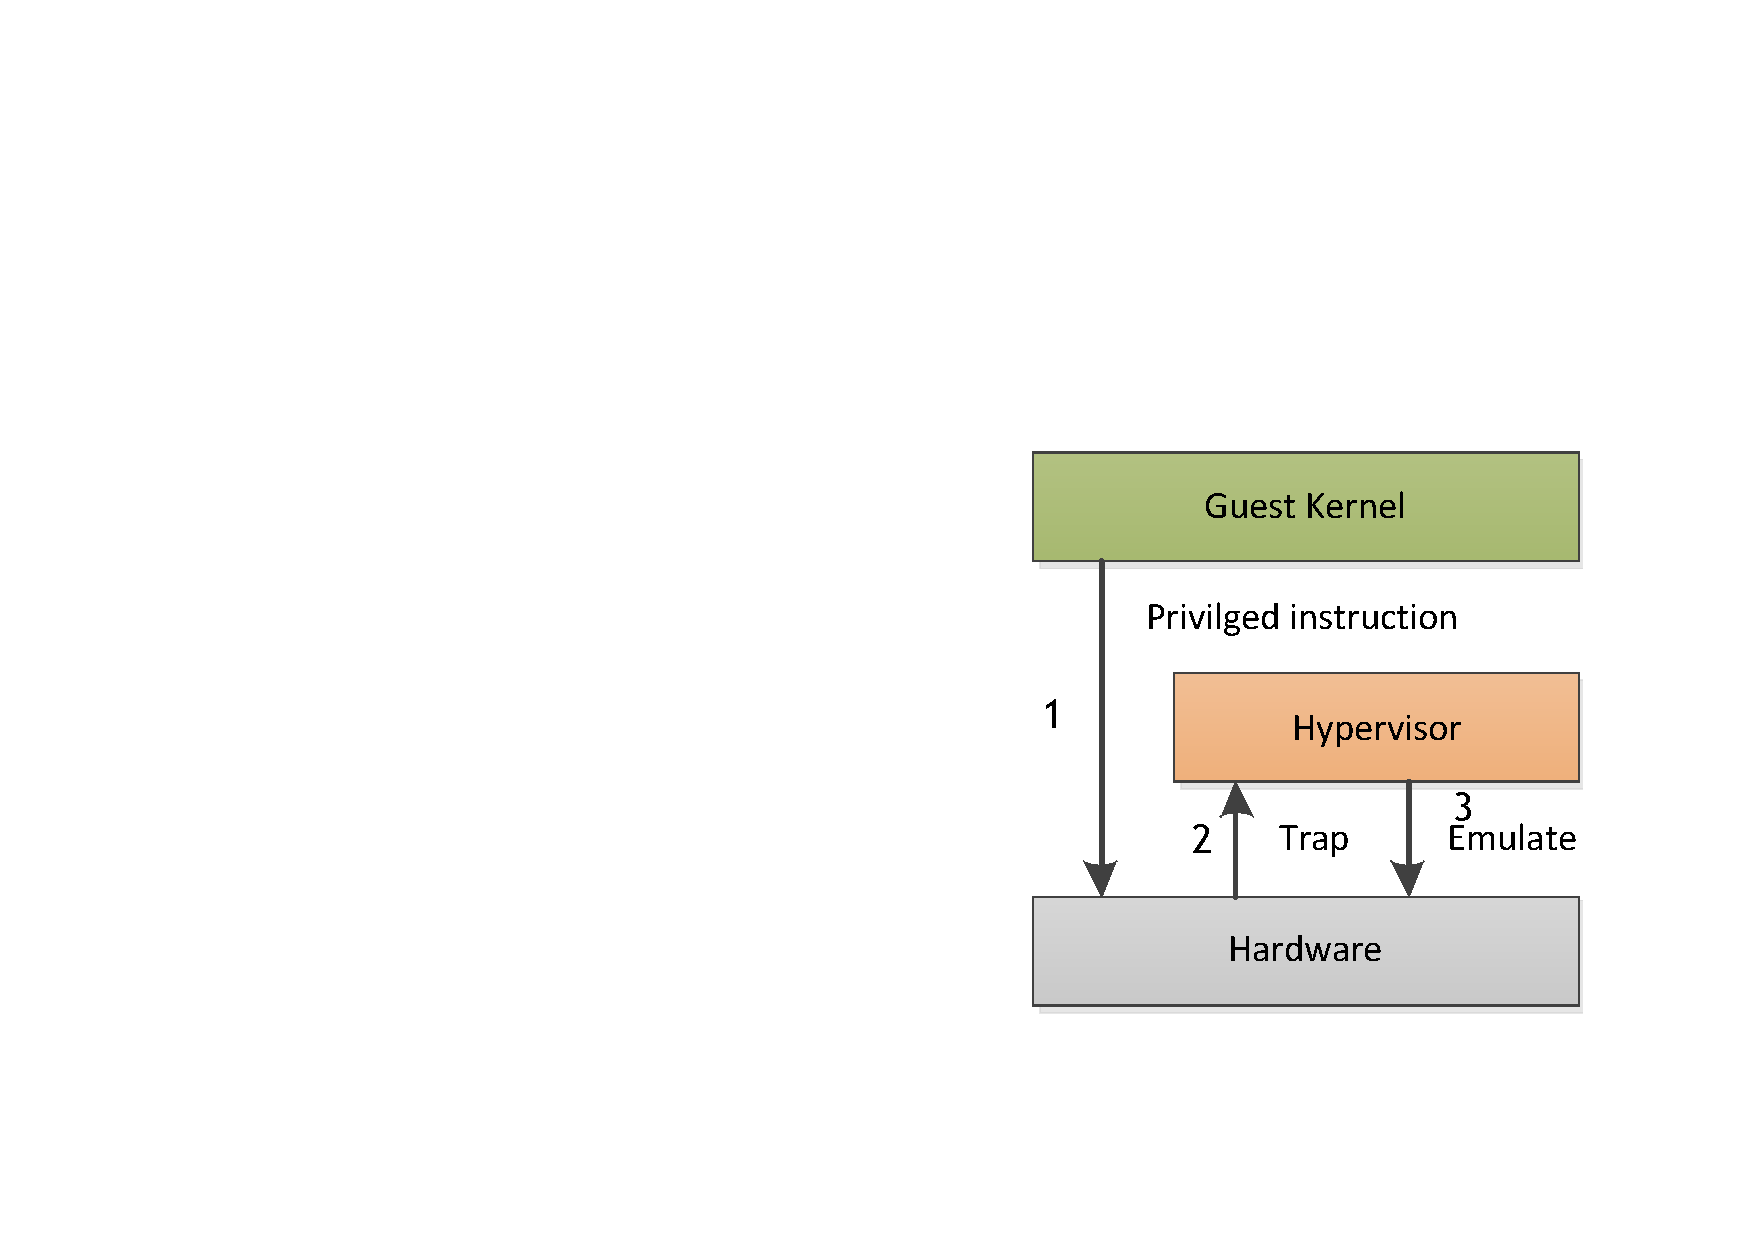
\includegraphics[width=.4\textwidth]{img/full-virtualization-2.pdf}
	\caption{Full Virtualization flow.}
\end{figure}

\longline

\paragraph{Paravirtualization}

\definition{Paravirtualization} \textbf{modifies the OS to use hypercalls instead of certain instructions}, making the process more efficient but requiring changes before compiling.

\highspace
Paravirtualization is a virtualization technique that uses hypercalls for operations to handle instructions at compile time. In paravirtualization, \emph{guest OS} is not completely isolated but it is partially isolated by the virtual machine from the virtualization layer and hardware. VMware and Xen are some examples of paravirtualization.

\highspace
Guest OS and VMM collaborates:
\begin{itemize}
	\item VMM present to VMs an interface similar but not identical to that of the underlying hardware.
	\item To reduce guest's executions of tasks too expensive for the virtualized environment (by means of \textbf{\dquotes{hooks} to allow the guest(s) and host to request and acknowledge tasks} which would otherwise be executed in the virtual domain, where execution performance is worse).
\end{itemize}

\highspace
\begin{flushleft}
	\textcolor{Green3}{\faIcon{check-circle} Advantages}
\end{flushleft}
\begin{itemize}
	\item \textbf{Simpler VMM}.
	\item \textbf{High Performance}.
\end{itemize}

\begin{flushleft}
	\textcolor{Red2}{\faIcon{thumbs-down} Disadvantages}
\end{flushleft}
\begin{itemize}
	\item \textbf{Modified Guest OS} (cannot be used with traditional OSs).
\end{itemize}

\newpage

\begin{figure}[!htp]
	\centering
	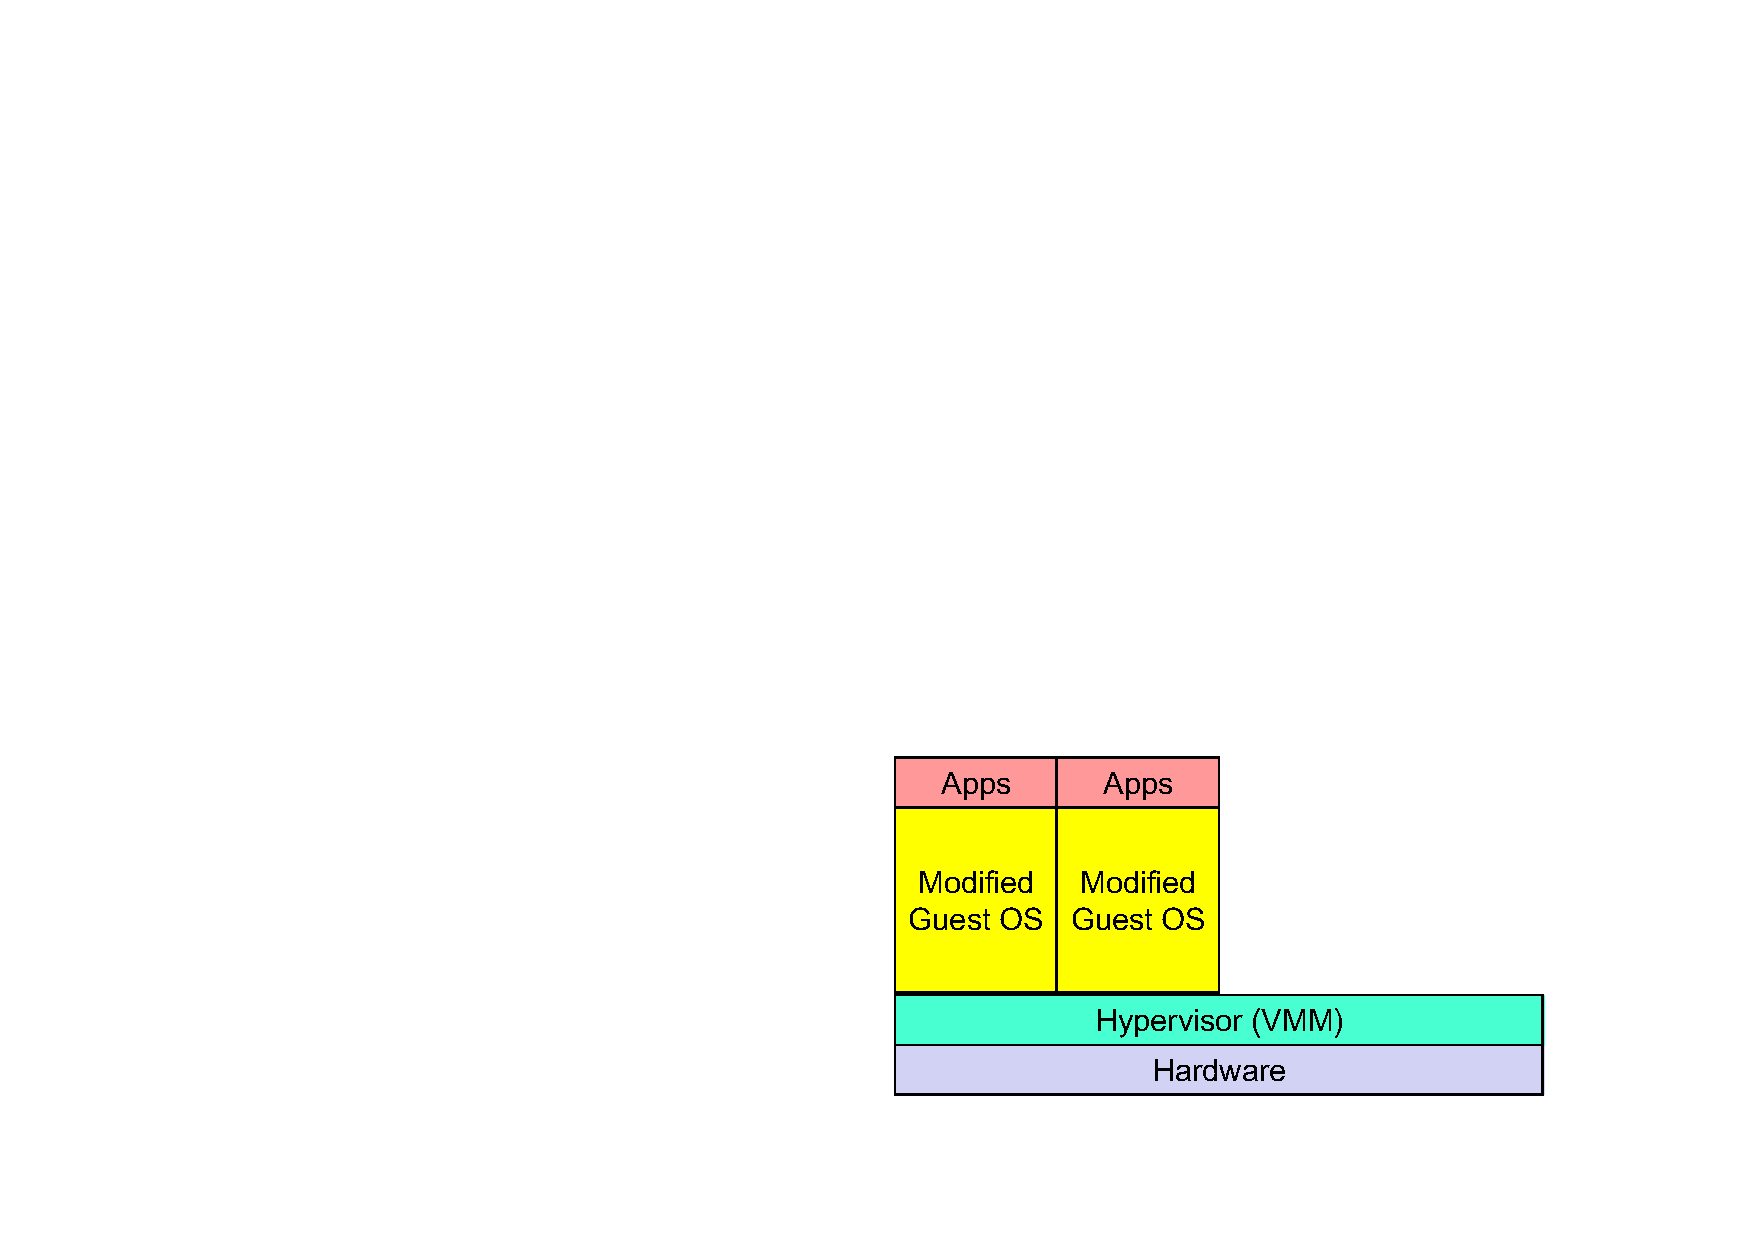
\includegraphics[width=.6\textwidth]{img/paravirtualization-1.pdf}
	\caption{View of the Paravirtualization.}
\end{figure}

\begin{figure}[!htp]
	\centering
	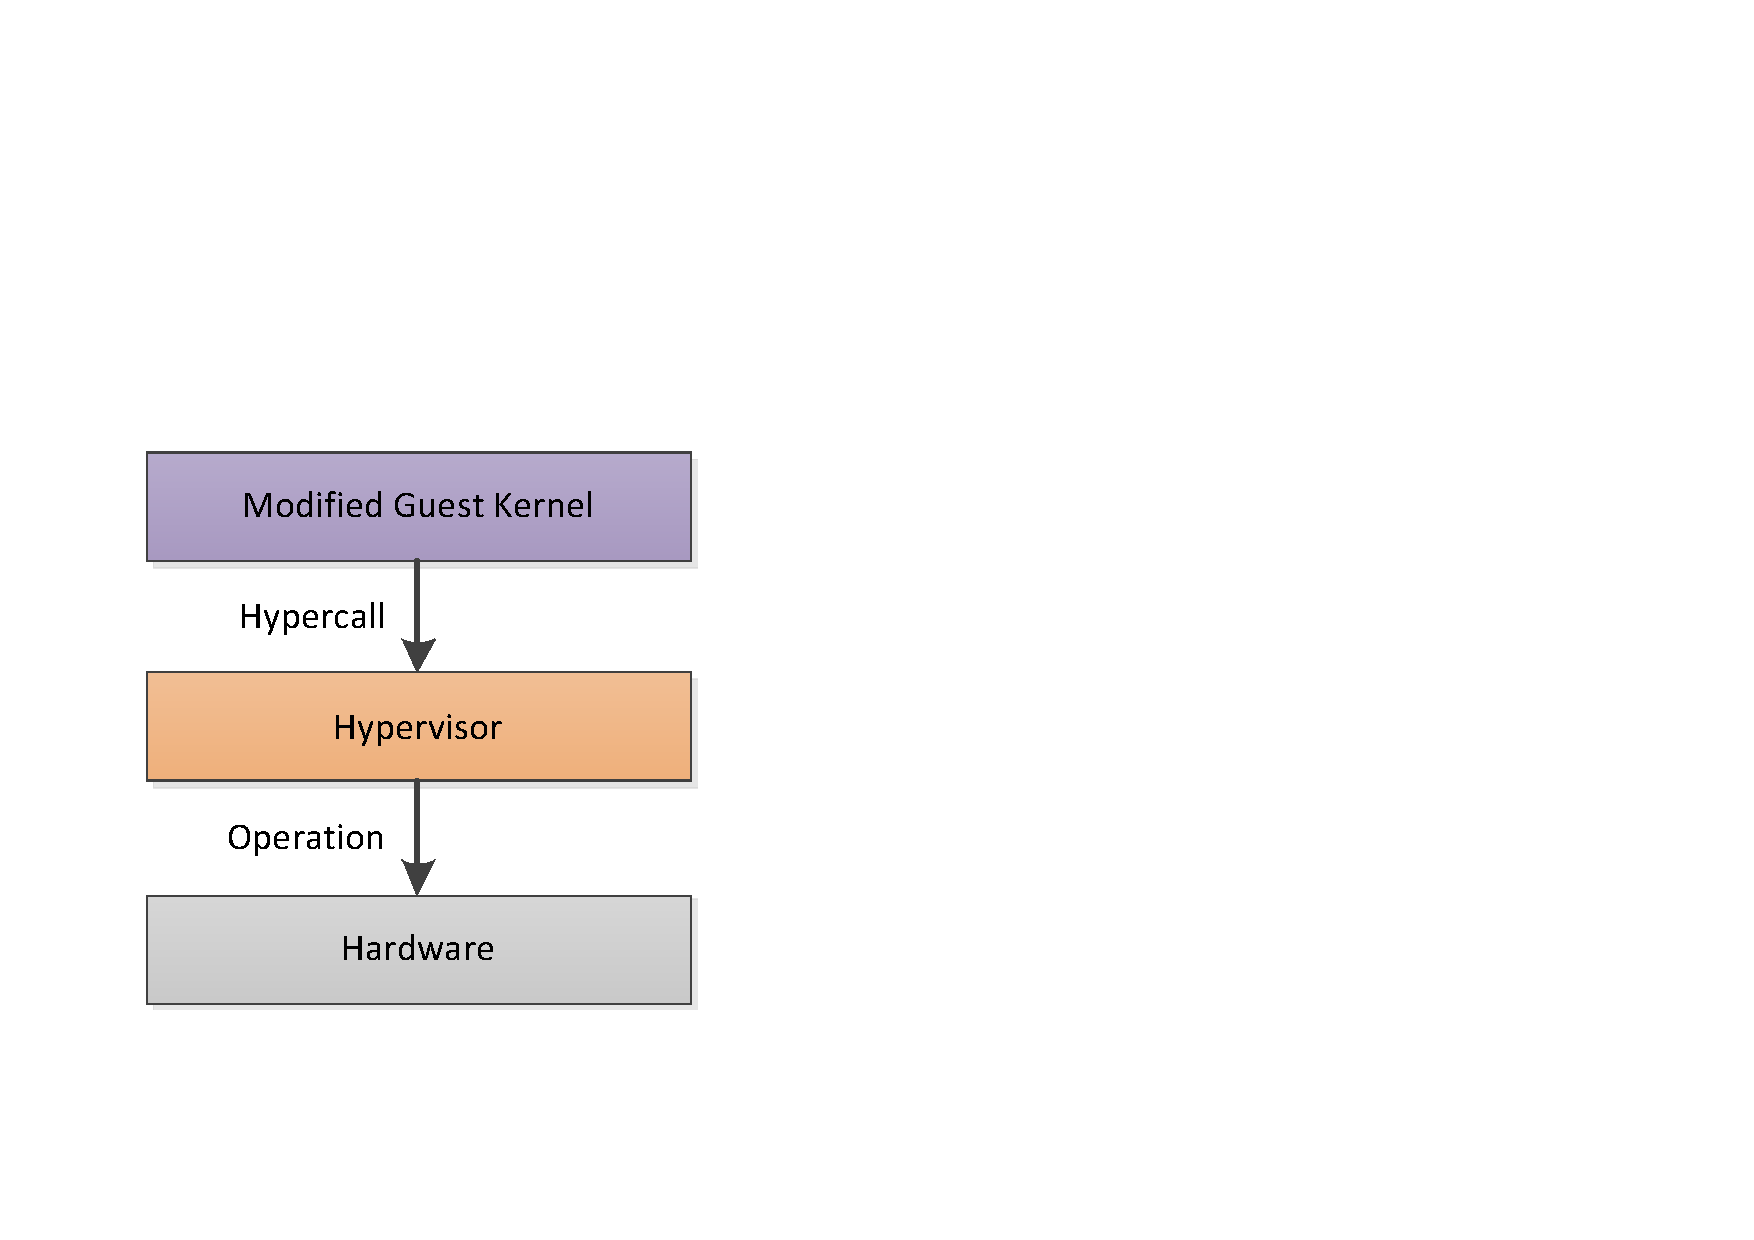
\includegraphics[width=.4\textwidth]{img/paravirtualization-2.pdf}
	\caption{Paravirtualization flow.}
\end{figure}

\newpage

\paragraph{Containers}

\definition{Container}s are \textbf{pre-configured packages}, with everything we need to execute the code (code, libraries, variables and configurations) in the target machine. Some well-known containers are Docker and Kubernetes.

\highspace
The \example{main advantage} of containers is that their \textbf{behavior is predictable}, \textbf{repeatable} and \textbf{immutable}. When we create a \dquotes{\emph{master}} container and duplicate it on another server, we know exactly how it will be executed. There are \textbf{no unexpected errors when moving it to a new machine or between environments}.

\begin{examplebox}
	If we have a container for a website, we do not need to export/import the dev/testing/production environments. We just create a container containing the site and move it to the target environment.
\end{examplebox}

\noindent
Virtual machine provides hardware virtualization, while \textbf{containers provide virtualization at the operating system level}. The \underline{main difference} is that the \textbf{containers share the host system kernel with other containers}.

\begin{figure}[!htp]
	\centering
	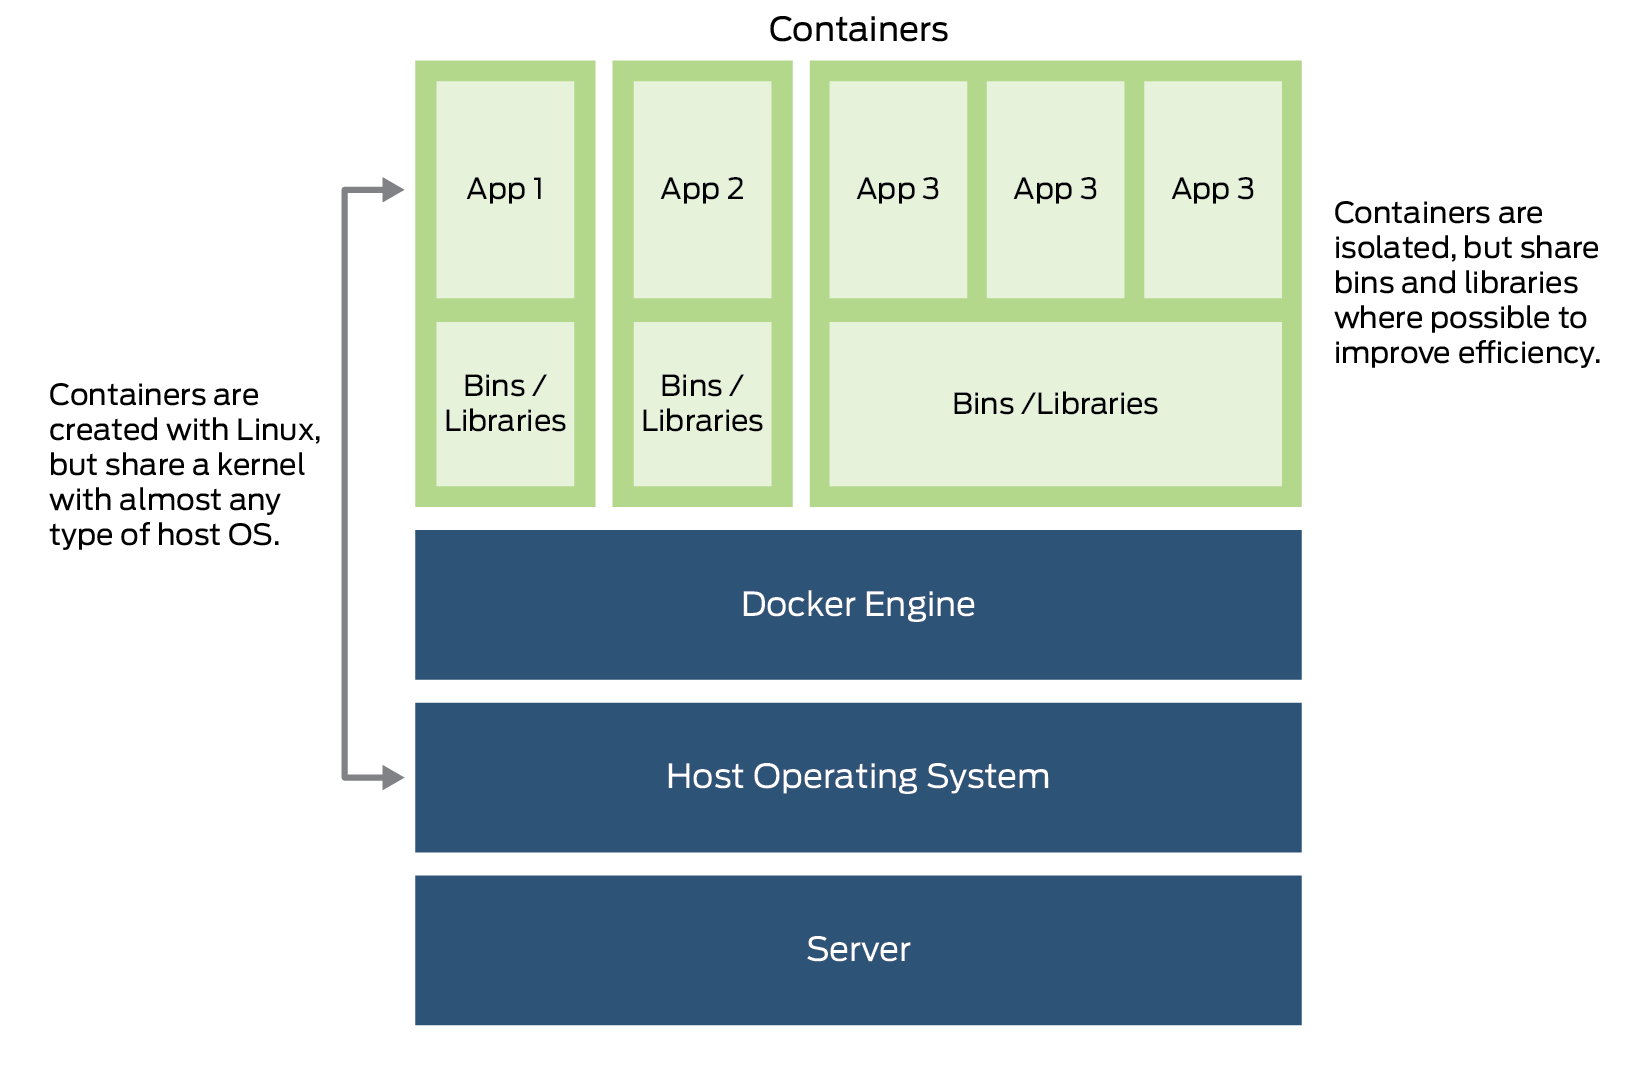
\includegraphics[width=\textwidth]{img/containers-1.png}
	\caption{Containers architecture.}
\end{figure}

\noindent
Some characteristics of containers:
\begin{itemize}
	\item \textbf{\underline{Flexible}}. Even the most complex application can be containerized.
	
	\item \textbf{\underline{Light}}. The containers exploit and share the host kernel.
	
	\item \textbf{\underline{Interchangeable}}. Updates can be distributed on the fly.
	
	\item \textbf{\underline{Portable}}. We can create locally, deploy in the cloud and run anywhere.
	
	\item \textbf{\underline{Scalable}}. It is possible to automatically increase and distribute replicas of the container.
	
	\item \textbf{\underline{Stackable}}. Containers can be stacked vertically and on the fly.
\end{itemize}
Containers ease the deployment of applications and increase the scalability but they also impose a \textbf{modular application development where the modules are independent and uncoupled}.

\highspace
\begin{flushleft}
	\textcolor{Green3}{\faIcon{question-circle} \textbf{Container Use Cases}}
\end{flushleft}
\begin{itemize}
	\item Make our \textbf{local development} and \textbf{build workflow faster}, more \textbf{efficient} and \textbf{lighter}.
	
	\item Run \textbf{standalone services and applications} consistently \textbf{across multiple environments}.
	
	\item Use \textbf{containers to create isolated instances to run tests}. For example, to create a db server SQL already configured to run tests.
	
	\item \textbf{Build and test complex applications and architectures on a local host} before deploying to a production environment.
	
	\item \textbf{Build a multi-user Platform-as-a-Service (PaaS) infrastructure}.
	
	\item Provide lightweight, stand-alone sandbox environments for developing, testing and teaching technologies such as the Unix shell or a programming language.
	
	\item \textbf{Software as a Service (SaaS) applications}.
\end{itemize}